\section{Value Based Temporal Regularization}
\label{sec:temp_reg}
%COMMENT(pierre-luc): "spatial" is not common terminology perhaps better to talk about regularization in feature space/state space, as in state abstraction vs temporal abstraction. Citations are also needed. Temporal regularization : could perhaps think of entropy-regularized work as a form of temporal regularization because it regularizes over pi_t and pi_{t+1}. You may also want to make it clear that "temporal regularization" is an expression coming from you, or otherwise provide citations. 
Regularization in the feature/state space, or \emph{spatial regularization} as we call it, exploits the regularities that exist in the observation (or state). In contrast, \emph{temporal regularization} considers the temporal structure of the value estimates through a trajectory. Practically this is done by smoothing the value estimate of a state using estimates of states that occurred earlier in the trajectory.
In this section we first introduce the concept of temporal regularization and discuss its properties in the policy evaluation setting. We then show how this concept can be extended to exploit information from the entire trajectory by casting temporal regularization as a time series prediction problem. 
\subsection{Definition}
Let us focus on the simplest case where the value estimate at the current state is regularized using only the value estimate at the previous state in the trajectory, yielding updates of the form % COMMENT(pierre-luc) : this sentence could be clearer. 
% Attempt: As a first step, we consider the case where the expected discounted return at a state also depends on the value at the previous step. 
% COMMENT(pierre-luc): You also need some more motivation as to why this particular form, especially the time-reversal aspect. Otherwise, it seems to be taken totally out of the blue. Why time-reversal matrix and not just P ? 
% COMMENT(pierre-luc) : "As a first step" suggests that you will introduce other forms of this operator in the paper. You do present the "time series" generalization, but don't develop it much further. So I would get rid of "first step", and start directly by explaining why incorporating previous values might be a good idea. 
\begin{equation}
    \begin{split}
        \Vr(s_{t}) &= \expect_{s_{t+1},s_{t-1} \sim \pi} [r(s_t) + \gamma ((1-\param)\Vr(s_{t+1}) + \param \Vr(s_{t-1}))]\\
         &= r(s_t) + \gamma (1-\param)\sum_{s_{t+1}\in \s} p(s_{t+1}|s_t)\Vr(s_{t+1})
         + \gamma \param \sum_{s_{t-1} \in \s}\frac{p(s_t|s_{t-1}) p(s_{t-1})}{p(s_t)} \Vr(s_{t-1}),
    \end{split}
\end{equation}
for a parameter $\param \in [0,1]$. It can be rewritten in matrix form as $\Vr = r + \gamma (((1-\param) P^{\pol} + \param \widetilde{P^{\pol}})\Vr) $, where $\widetilde{P^{\pol}}$ corresponds to the reversal Markov chain of the MDP.
We define a temporally regularized Bellman operator as:
\begin{equation}
\label{eqn:temp_reg_bellman_op}
    \regT v_{\param} = r + \gamma ((1-\param) P^{\pol}v_{\param} + \param \widetilde{P^{\pol}} v_{\param}).
\end{equation}
To alleviate the notation, we denote $P^{\pol}$ as $P$ and $\widetilde{P^{\pol}}$ as $\widetilde{P}$.
\begin{remark}
For $\param =0$, Eq.~\ref{eqn:temp_reg_bellman_op} corresponds to the original Bellman operator.
\end{remark}
We can prove that this operator has a unique fixed point, $\Vr^{\pol}$.
%COMMENT(pierre-luc): I would just splash Theorem 1 without stating Lemma 1 (which is just one line and isn't proved). You can instead mention it in the proof, and give a reference for this fact.
% \begin{lemma}
% \label{lem:stochastic_matrix_convex_combination}
% The convex combination of two row stochastic matrices is also row stochastic.
% \end{lemma}
\begin{theorem}
The operator $\regT$ has a unique fixed point $\Vr^{\pol}$ and $\regT$ is a contraction mapping.
\end{theorem}
\begin{proof}
We first prove that $\regT$ is a contraction mapping in $L_\infty$ norm. We have that
\begin{equation}
\begin{split}
    \norm{\regT u - \regT v}_{\infty} &= \norm{r+\gamma( (1-\param) Pu + \param \widetilde{P}u) - (r+\gamma( (1-\param) Pv + \param \widetilde{P}v))}_{\infty}\\
    &= \gamma \norm{((1-\param) P + \param \widetilde{P})(u-v)}_{\infty}\\
    &\leq \gamma \norm{u-v}_{\infty},
\end{split}
\end{equation}
where the last inequality uses the fact that the convex combination of two row stochastic matrices is also row stochastic (he proof can be found in the appendix).
%is obtained with Lemma~\ref{lem:stochastic_matrix_convex_combination}.
Then using Banach fixed point theorem, we obtain that $\Vr^{\pol}$ is a unique fixed point. 
\end{proof}
\begin{algorithm}[H]
\caption{Policy evaluation with temporal regularization}
\begin{algorithmic}[1]
    \STATE Input: $\pi,\alpha,\gamma,\param,\lambda$
    \STATE $p = V(s)$
    \FORALL{steps}
        \STATE Choose $a \sim \pi(\s)$
        \STATE Take action $a$, observe $r(s),s'$
        \STATE $\V(s) = r(s) + \gamma ( (1-\param) \V(s') + \param p) $
        \STATE $p = \V(s) $
    \ENDFOR
\end{algorithmic}
\label{alg:pol_eval_exp_smoothing}
\end{algorithm}

Furthermore the new induced Markov chain $(1-\param) P + \param \widetilde{P}$ has the same stationary distribution as the original $P$ (the proof can be found in the appendix).
\begin{lemma}
\label{cor:same_stationary_dist}
$P$ and $(1-\param) P + \param \widetilde{P}$ have the same stationary distribution $\mu \quad \forall \param \in [0,1]$.
\end{lemma}
%COMMENT(pierre-luc): $P$ and $(1-\param) : order is confusing. I would write something like:
% The stationary distribution induced by $(1-\param) P + \param \widetilde{P}$ is $\mu$: the stationary distribution under the original Markov chain $P$.


%COMMENT(pierre-luc): You first need to start this paragraph by saying that there is indeed a bias, because this is not something that you would expect from a "regular" policy evaluation operator. Then quickly reinsure the reader that this bias is not evil because the resulting operator as some desirable properties : a knob for variance reduction. 
\subsection{Bias}
In the policy evaluation setting, the bias between the original value function $\V^{\pol}$ and the regularized one $\V^{\pol}_{\param}$ can be characterized as a function of the difference between $P$ and its Markov reversal $\widetilde{P}$, weighted by $\param$ and the reward distribution.

%COMMENT(pierre-luc) : Minor notational preference in favor of "t" instead of "i". 
%COMMENT(pierre-luc): You need to say that these Neumann series converge. This follows from your contraction argument above. You can state Puterman corollary C.4 for the existence of the series and its inverse. 
%COMMENT(pierre-luc): A general statement for all LP norms ? If not, or generality is not needed, stick to more common sup/infinity norm. 
\begin{property}
Let $v^{\pol} = \sum_{i=0}^{\infty} \gamma^i P^i r$ and $v^{\pol}_{\param} = \sum_{i=0}^{\infty} \gamma^i ((1-\param) P + \param \widetilde{P})^i r$. We have that
\begin{equation}
    \begin{split}
        \norm{v^{\pol} - v^{\pol}_{\param}}_p &= \norm{\sum_{i=0}^{\infty} \gamma^i (P^i-((1-\param) P + \param \widetilde{P})^i) r}_p \\
        &\leq \sum_{i=0}^{\infty} \gamma^i \norm{ (P^i-((1-\param) P + \param \widetilde{P})^i) r}_p.
    \end{split}
\end{equation}
This quantity is naturally bounded for $\gamma < 1$.
\end{property}
\begin{remark}
Let $P^\infty$ denote a matrix where columns consist of the stationary distribution $\mu$.
By the property of reversal Markov chains and lemma \ref{cor:same_stationary_dist}, we have that $\lim_{i\rightarrow\infty} \Vert P^i r-P^\infty r \Vert \rightarrow 0$ and $\lim_{i\rightarrow\infty} \Vert ((1-\param)P+\param \widetilde{P})^i r-P^\infty r \Vert \rightarrow 0$, such that the Marvov chain $P$ and its reversal $(1-\param)P+\param \widetilde{P}$ converge to the same value. Therefore, the norm $\Vert  (P^i-((1-\param) P + \param \widetilde{P})^i) r \Vert_p$ also converges to 0 in the limit.
\end{remark}

\begin{remark}
It can be interesting to note that if the chain is reversible, meaning that $P = \widetilde{P}$, then the fixed point of both operators is the same, that is $v^\pol = v_\param^\pol$.
\end{remark}

\subsection{Variance}
If the chain is reversible than I can find a factor of 2 on the variance because you just get twice more sample. In the non reversible case same thing. If you were to be able to sample from the newly generated $P_{\param}$ then you would solve it half as fast. Could be a cool argument.
\subsection{Average reward case:} The temporally regularized MDP has the same average reward as the original one as it is possible to define the average reward \cite{tsitsiklis2002average} as a function of the stationary distribution $\pi$, the reward vector and $\gamma$ . This leads to the following property (the proof can be found in the appendix).

\begin{property}
For a reward vector r, the MDPs defined by the the transition matrices $P$ and $(1-\param) P + \param \widetilde{P}$ have the same average reward $\rho$.
\end{property}
Intuitively this means that temporal regularization only reweigh the reward on each state based on the Markov reversal while preserving the average reward.

%COMMENT(pierre-luc): You could also call this section "Higher Order Temporal Regularization". In RLS/ARMA/signal processing, I think they refer to the "order" of their filter when they incorporate older information. See LTI filters.
\subsection{Temporal Regularization as a time series prediction problem:}
It is possible to cast this problem of temporal regularization as a time series prediction problem and use richer models of temporal dependencies, such as exponential smoothing \cite{gardner2006exponential}, ARMA model~\cite{box94}, etc. We can write the update in a general form using $n$ different regularizers ($\widetilde{v_0},\widetilde{v_1}...\widetilde{v_{n-1}}$):
\begin{equation}
    \V(s_t) = r(s) + \gamma \sum_{i=0}^N [\param(i) \widetilde{\V}_i(s_{t+1})],
\end{equation}
where $\widetilde{\V}_0(s_{t+1}) = \V(s_{t+1})$ and $\sum_{i=0}^N \param(i) = 1$. For example, using exponential smoothing where $\widetilde{\V}(s_{t+1}) = (1-\lambda) \V(s_{t-1}) + (1-\lambda)\lambda \V(s_{t-2})...$, the update can be written in operator form as:
\begin{equation}
    \regT v = r + \gamma \bigg(\left(1-\param\right) Pv + \param \left(1-\lambda\right) \sum_{i=1}^{\infty} \lambda^{i-1} \widetilde{P}^i v\bigg),
\end{equation}
and a similar argument as Theorem 1 can be used to show the contraction property.

Using more powerful regularizers could be beneficial, for example to reduce variance by smoothing over more values (exponential smoothing) or to model the trend of the value function through the trajectory (trend adjusted model). An example a temporal policy evaluation with temporal regularization using exponential smoothing can be found in the appendix.
\begin{algorithm}[H]
\caption{Policy evaluation with exponential smoothing}
\begin{algorithmic}[1]
    \STATE Input: $\pi,\alpha,\gamma,\param,\lambda$
    \STATE $p = V(s)$
    \FORALL{steps}
        \STATE Choose $a \sim \pi(\s)$
        \STATE Take action $a$, observe $r(s),s'$
        \STATE $\V(s) =  r(s) + \gamma ( (1-\param) \V(s') + \param p) $
        \STATE $p = (1-\lambda)\V(s) + \lambda p$
    \ENDFOR
\end{algorithmic}
\label{alg:pol_eval_exp_smoothing}
\end{algorithm}
%COMMENT(pierre-luc) : It feels too disconnected from the flow. I would just move this to the conclusion as future work. 
\subsection{Control} 
Temporal regularization can be extended to control by  modifying the target of the value function (or the Q values) using temporal regularization. Experiments (Sec.~\ref{sec:expe:drl}) present an example of how temporal regularization can be applied within an actor-critic framework. The theoretical analysis of the control case is outside the scope of this paper.

\subsection{Temporal difference with function approximation}
It is also possible to extend temporal regularization using function approximation such as  semi-gradient TD \cite{sutton2017reinforcement}. 
%COMMENT(pierre-luc): Semi-gradient is a new terminology introduced in the draft of the new S&B textbook. Not found in 1998
Assuming a function $\V_{\theta}^{\param}$ parameterized by $\theta$, we can consider $r(s) + \gamma ((1-\param)\V_{\theta}^{\param}(s_{t+1}) + \param \V_{\theta}^{\param}(s_{t-1})) - \V_{\theta}^{\param}(s_t)$  as the target and differentiate with respect to $\V_{\theta}^{\param}(s_{t})$. An example of a temporally regularized semi-gradient TD algorithm can be found in the appendix.
%COMMENT(pierre-luc) : I would include this in the main text + pseudo-code. Important to show that the MDP formulation can be efficiently translated into a usable model-free algorithm. The time-reversibility would be a concern for me if I were to review this paper and it hadn't be addressed by this point yet. 


\begin{algorithm}[H]
\caption{Temporally regularized semi-gradient TD}
\begin{algorithmic}[1]
    \STATE Input: policy $\pi$,$\param$,$\gamma$
    \FORALL{steps}
        \STATE Choose $a \sim \pi(s_t)$
        \STATE Take action $a$, observe $r(s),s_{t+1}$
        \STATE $\theta = \theta + \alpha (r + \gamma((1-\param) \V_{\theta}(s_{t+1}) + \param \V_{\theta}(s_{t-1})) - \V_{\theta}(s_t))\nabla \V_{\theta}(s_{t}) $
    \ENDFOR
\end{algorithmic}
\end{algorithm}

\begin{property}
For a reward vector r, the MDP defined by the the transition matrix $P$ and $(1-\param) P + \param \widetilde{P}$ have the same average reward $\rho$.
\begin{equation}
    \frac{\rho}{1-\alpha} = \sum_i^{\infty}\gamma^i \pi^T r.
\end{equation}
\end{property}

\begin{lemma}
$P$ and $(1-\param) P + \param \widetilde{P}$ have the same stationary distribution $\mu \quad \forall \param \in [0,1]$.
\end{lemma}
\begin{proof}
It is known that $P^{\pol}$ and $\widetilde{P^{\pol}}$ have the same stationary distribution. Using this fact we have that
\begin{equation}
    \begin{split}
        \mu( (1-\param) P^{\pol} + \param \widetilde{P^{\pol}}) &=  (1-\param) \mu P^{\pol} + \param \mu \widetilde{P^{\pol}} \\
        &= (1-\param)\mu + \param \mu\\
        &= \mu.
    \end{split}
\end{equation}
\end{proof}

\begin{lemma}
\label{lem:stochastic_matrix_convex_combination}
The convex combination of two row stochastic matrices is also row stochastic.
\end{lemma}
\begin{proof}
Let e be vector a columns vectors of 1.
\begin{equation}
\begin{split}
       (\param P^{\pol} + (1-\param) \widetilde{P^{\pol}})e &= \param P^{\pol}e +  (1-\param) \widetilde{P^{\pol}}e \\
       &= \param e + (1-\param) e\\
       &= e.
\end{split}
\end{equation}
\end{proof}
\subsection{Connection with multi-step methods}

\section{Experiments}


We now presents empirical results illustrating potential advantages of temporal regularization, and characterizing its bias and variance effects on value estimation and control.



\subsection{Mixing time}
This first experiment showcases that the underlying Markov chain of a MDP can have a smaller mixing time when temporally regularized. The mixing time can be seen as the number of time steps required for the Markov chain to get \emph{close enough} to its stationary distribution. Therefore, the mixing time also determines the rate at which policy evaluation will converge to the optimal value function~\cite{baxter2001infinite}. 
%COMMENT(pierre-luc) : can also cite Puterman, spectral radius. Also, not just for control (you say "optimal") : also true for policy evaluation.
%COMMENT(pierre-luc): Mixing quickly is one thing, but mixing quickly and returning an answer not too far away from the actual answer (bias) is very important. When reading this paragraph, I would need to convince myself that this is not a vacuous demonstration, that the resulting fast-mixing chain is still somewhat related to the original problem.
We consider a synthetic MDP with 10 states where transition probabilities are sampled from the uniform distribution. Let $P^{\infty}$ denote a matrix where columns consists of the stationary distribution $\mu$. To compare the mixing time, we evaluate the error corresponding to the distance of $P^i$ and $\big((1-\param)P+\param \widetilde{P}\big)^i$ to the convergence point $P^{\infty}$ after $i$ iterations.
%
Figure~\ref{fig:mixing} displays the error curve when varying the regularization parameter $\param$. We observe a U-shaped error curve, that intermediate values of $\param$ in this example yields faster mixing time.
\begin{figure}
    \centering
    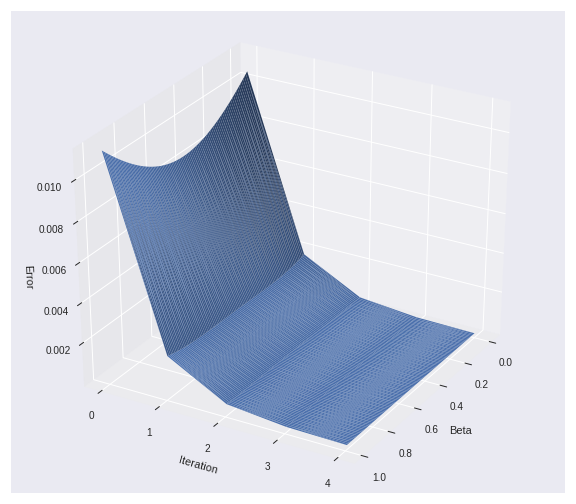
\includegraphics[scale=0.5]{fig/Markov_mixing.png}
    \caption{Distance between the stationary transition probabilities and the estimated transition probability for different values of regularization parameter $\param$.}
    \label{fig:mixing}
\end{figure}
One explanation is that transition matrices with extreme probabilities (low or high) yield poorly conditioned transition matrices. Regularizing with the reversal Markov chain often leads to a better conditioned matrix at the cost of injecting bias.
%COMMENT(pierre-luc) : poorly conditioned: you should compute the actual condition numbers to convince the reader that this is actually what is happening. 

\subsection{Bias}
\label{sec:expe:bias}

It is well known that reducing variance comes at the expense of inducing (smaller) bias.
%COMMENT(pierre-luc): citation still needed. You can perhaps cite general ML textbooks such as Hastie ESL or Bishop. You can also cite  Bertsekas (2012) and Satinder Singh and Kearns for bias-variance of TD(lambda).
This has been characterized previously (Sec.~\ref{sec:temp_reg}) in terms of the difference between the original Markov chain and the reversal weighted by the reward. In this experiment, we attempt to give an intuitive idea of what this means. More specifically, we would expect the bias to be small if values along the trajectories have similar values.
To this end, we consider a synthetic MDP with $10$ states where both transition functions and rewards are sampled randomly from a uniform distribution. In order to create temporal dependencies in the trajectory, we smooth the rewards of $N$ states that are temporally close (in terms of trajectory) using the following formula: $ r(s_t) = \frac{r(s_t) + r(s_{t+1})}{2}$.
Figure~\ref{fig:mod} shows the difference between the regularized and un-regularized MDPs as $N$ changes, for different values of regularization parameter $\param$.
\begin{figure}
    \centering
    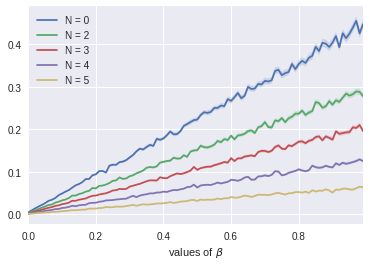
\includegraphics[scale=0.8]{fig/mod.png}
    \caption{Mean difference between $\Vr^{\pi}$ and $\V^{\pi}$ given the regularization parameter $\param$, for different amount of smoothed states $N$.}
    \label{fig:mod}
\end{figure}
We observe that increasing $N$, meaning more states get rewards close to one another, results into less bias. This is due to rewards putting emphasis on states where the original and reversal Markov chain are similar.

\subsection{Variance number 2}
You could use a random walk. The P is reversible to so no bias. Then compare the performance of monte carlo, TD and our thing. Should just be faster. In this case you want to compare with the number of samples used and try to show an increase of 2 folds. its like having double the sample link the variance from theory before

\subsection{Variance}
\label{sec:expe:variance}
% COMMENT(pierre-luc) : this should be emphasized earlier.
The primary motivation of this work is to reduce variance, therefore we now consider an experiment  targeting this aspect. Figure~\ref{fig:MDP} shows an example of a synthetic, three states MDP, where the variance of $S_1$ is (relatively) high.
\begin{figure}
    \centering
    \includegraphics[scale=0.7]{fig/Exp_2.png}
    \caption{Synthetic MDP where state $S_1$ has high variance.}
    \label{fig:MDP}
\end{figure}
We consider an agent that is evolving in this world, changing states following the stochastic policy indicated. We are interested in the error when estimating the optimal state value of $S_1$, $\V^*(S_1)$, with and without temporal regularization, denoted $\Vr^{\pi}(S_1)$, $\V^{\pi}(S_1)$, respectively.

Figure~\ref{fig:perf_MDP} shows these errors at each iteration, averaged over $100$ runs. We observe that temporal regularization indeed reduces the variance and thus helps the learning process by making the value function easier to learn.
\begin{figure}
    \centering
    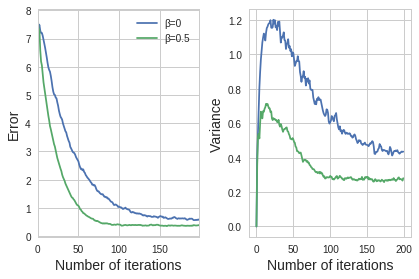
\includegraphics[scale=0.7]{fig/exp_2_result.png}
    \caption{Left plot showsabsolute difference between original ($\V^{\pi}(S_1)$) and regularized ($\Vr^{\pi}(S_1)$) state value estimates to the optimal value $\V^*(S_1)$. Right plot shows the variance of the estimates $\V$.}
    \label{fig:perf_MDP}
\end{figure}

\subsection{Propagation of the information}
We now illustrate with a simple experiment how temporal regularization allows the information to spread faster among the different states of the MDP. For this purpose, we consider a simple MDP, where an agent walks randomly in two rooms (18 states) using four actions (up, down, left, right), and a discount factor $\gamma=0.9$. The reward is $r_t=1$ everywhere and passing the door between rooms (shown in red on Figure~\ref{fig:room}) only happens 50\% of the time (on attempt). The episode starts at the top left and terminates when the agent reaches the bottom right corner. The sole goal is to learn the optimal value function by walking along this MDP (this is not a race toward the end).

Figure~\ref{fig:room} shows the proximity of the estimated state value to the optimal value with and without temporal regularization. The darker the state, the closer it is to its optimal value. The heatmap scale has been adjusted at each trajectory to observe the difference between both methods.
We first notice that the overall propagation of the information in the regularized MDP is faster than in the original one. We also observe that, when first entering the second room, bootstrapping on values coming from the first room allows the agent to learn the optimal value faster. This suggest that temporal regularization could help agents explore faster by using their prior from the previous visited state for learning the corresponding optimal value faster.

\begin{figure}
    \centering
    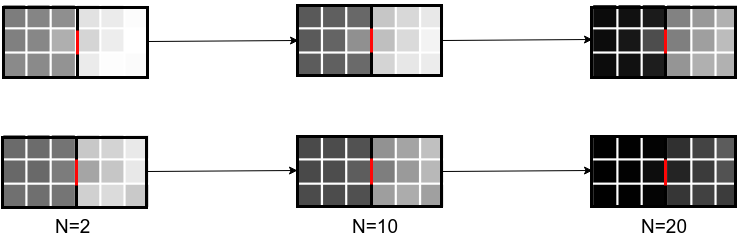
\includegraphics[scale=0.44]{fig/room.png}
    \caption{Proximity of the estimated state value to the optimal value after $N$ trajectories. Top row is the original room environment and bottom row is the regularized one ($\param = 0.5$). Darker is better.}
    \label{fig:room}
\end{figure}


\subsection{Noisy state representation}
\label{sec:expe:noisy_state}

The next experiment illustrates a major strength of temporal regularization, that is its robustness to noise in the state representation. This situation can naturally arise when the state sensors are noisy or insufficient to avoid aliasing.
\begin{figure}
    \centering
    
\includegraphics[scale=0.7]{fig/random_walk.png}
    \caption{Synthetic, one dimensional, MDP where the reward corresponds to the position of the agent in $[0, 1]$.}
    \label{fig:MDP_noisy}
\end{figure}
For this task, we consider the synthetic, one dimensional, continuous setting displayed in Figure~\ref{fig:MDP_noisy}. A learner evolving in this environment walks randomly along this line with a discount factor $\gamma=0.5$. Let $x_t\in [0,1]$ denote the position of the agent along the line at time $t$. The next position $x_{t+1} = x_t + a_t$, where action $a_t\sim\mathcal{N}(0, 0.1)$. The state of the agent corresponds to the position perturbed by a zero-centered Gaussian noise $\epsilon_t$, such that $s_t = x_t + \epsilon_t$, where $\epsilon_t\sim\mathcal{N}(0,\sigma^2)$ are i.i.d. When the agent moves to a new position $x_{t+1}$, it receives a reward $r_t = x_{t+1}$. The episode ends after 100 steps. In this experiment we model the value function using a linear model with a single parameter $\theta$. We are interested in the error when estimating the optimal parameter function $\theta^*$ with and without temporal regularization, that is $\theta^\pi_\param$ and $\theta^\pi$, respectively. In this case we use the TD version of temporal regularization presented at the end of Sec.~\ref{sec:temp_reg}.
\begin{figure}
    \centering
    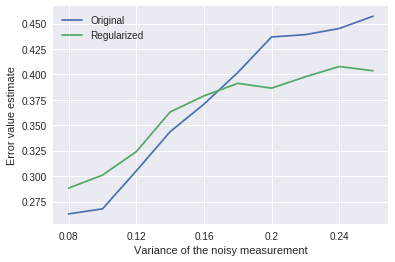
\includegraphics[scale=0.7]{fig/spatial_temporal.png}
    \caption{Absolute distance from the original ( $\theta^\pi$) and the regularized ($\theta^\pi_\param$) state value estimates to the optimal parameter $\theta^*$ given the noise variance $\sigma^2$ in state sensors.}
    \label{fig:perf_MDP_noisy}
\end{figure}
Figure~\ref{fig:perf_MDP_noisy} shows these errors, averaged over 100 repetitions, for different values of noise variance $\sigma^2$. We observe that as the noise variance increases, the un-regularized estimate becomes less accurate, while temporal regularization is more robust. This experiment highlights a case where temporal regularization is effective even in the absence of smoothness in the state space (which other regularization methods would target). This is further highlighted in the next experiments.



\subsection{Deep reinforcement learning}
\label{sec:expe:drl}

To showcase the potential of temporal regularization in high dimensional settings, we adapt an actor-critic based method (PPO \cite{schulman2017proximal}) using temporal regularization. More specifically, we incorporate temporal regularization as exponential smoothing in the target of the critic. 
% COMMENT(pierre-luc): Atari games: we evaluate the performance in the Arcade Learning Environment (ALE), citation Bellemare 2011 or 2013 ? 
We evaluate the performance on multiple Atari games, where we consider the following performance measure \cite{xu2017natural}:
\begin{equation}
\label{eqn:expe:drl_measure}
    \frac{\text{regularized} - \text{baseline}}{\text{baseline} - \text{random}}.
\end{equation}
%COMMENT(pierre-luc) : what is "baseline", plain PPO that you re-ran or other reported algorithm ?
The hyper-parameters for the temporal regularization are $\param = 0.2$ and a decay of $1\mathrm{e}^{-5}$. Those are selected on 7 games and 3 training seeds. All other hyper-parameters correspond to the one used in the PPO paper. Our implementation\footnote{The code can be found in the supplementary material.} is based on the publicly available OpenAI codebase~\cite{baselines}. The previous four frames are considered as the state representation~\cite{mnih2015human}.
For each game, $10$ independent runs ($10$ random seeds) are performed and the performance are reported in Figure~\ref{fig:graph_atari}. 


Figure~\ref{fig:graph_atari} shows that adding temporal regularization improves the performance on multiple games. This suggests that the regularized optimal value function may be smoother and thus easier to learn, even when using function approximation with deep learning. Also, as shown in previous experiments (Sec.~\ref{sec:expe:noisy_state}), temporal regularization being independent of spatial representation makes it more robust to mis-specification of the state features, which is a challenge in some of these games (e.g. when assuming full state representation using some previous frames).

\begin{figure}
    \centering
    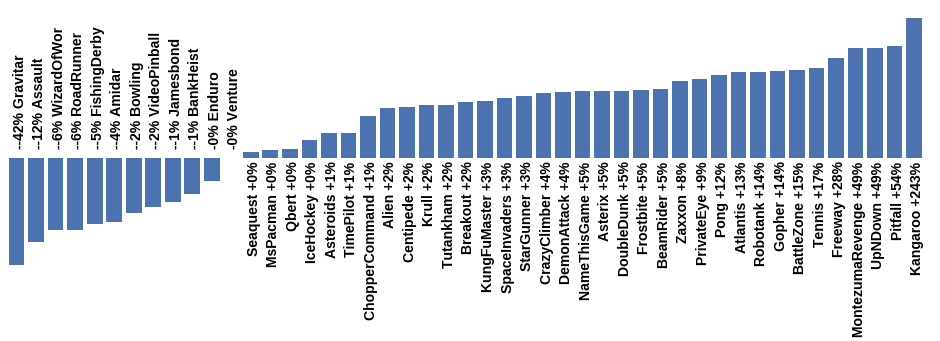
\includegraphics[width=13cm,height=4cm]{fig/bar_atari.png}
    \caption{Performance (Eq.~\ref{eqn:expe:drl_measure}) of a temporally regularized PPO on a suite of Atari games.}
    \label{fig:graph_atari}
\end{figure}

\begin{figure}
    \centering
    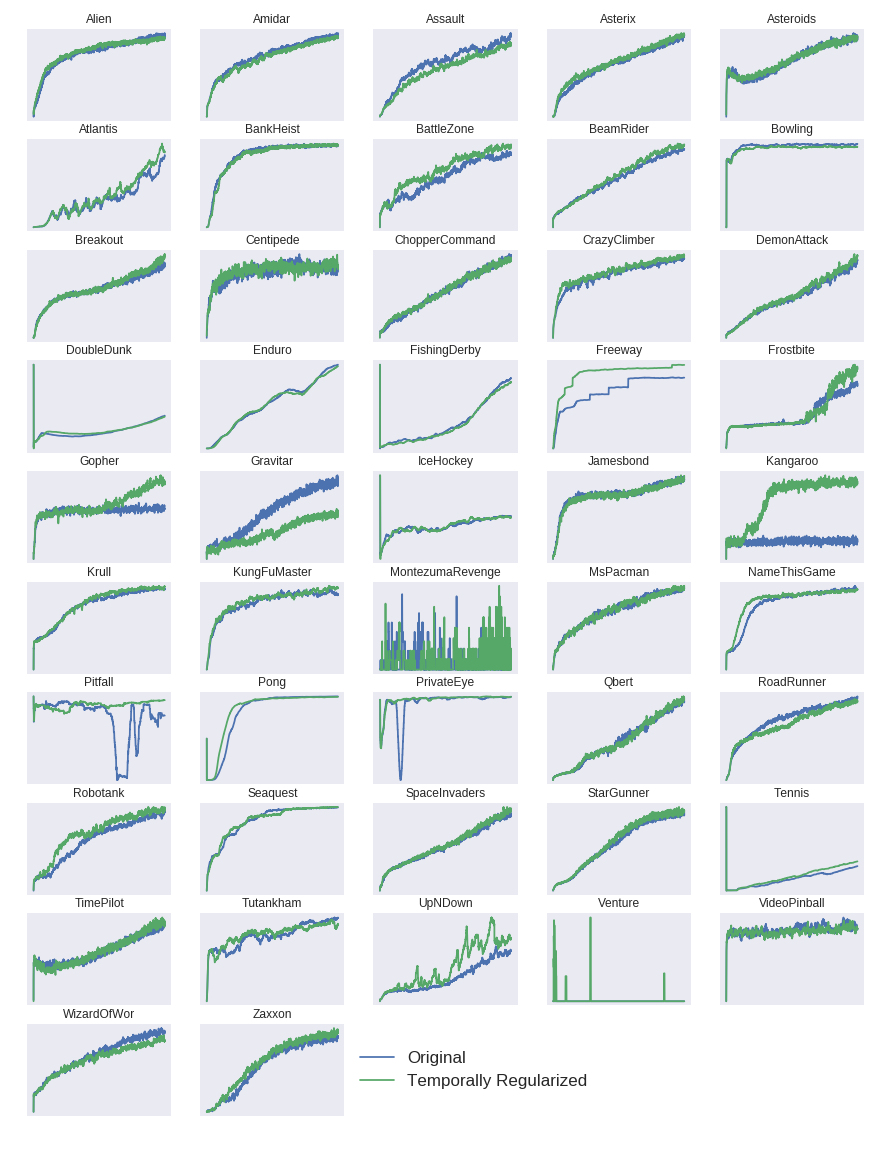
\includegraphics[scale=0.5]{fig/plot_atari.png}
    \caption{Average reward per episode on Atari games.}
    \label{fig:my_label}
\end{figure}
\section{Policy Gradient Temporal Regularization}

This idea is a continuation of the paper I wrote recently about what I call “Temporal Regularization”. The main intuition is to exploit previous estimate (v, q or pi’s) along the trajectory to reduce the variance of the current estimate. In particular in this project we are interested in policy gradient. We want to regularize the objective function by constraining the policy to be more "consistent" temporally 
\begin{equation}
\begin{split}
    R(\pi) = \beta ( \pi(a_{t-1}|s_{t-1}) - \pi(a_t|s_t)) \\
\end{split}
\end{equation}
It is possible to see this formulation as some kind of entropy regularization where the regularization is done in trajectory space compared to PPO ect… where it is done in policy space. Another perspective is to view $\pi$ as a time series and apply some entropy regularization to the prediction of the time series. Some of the advantages of doing this kind of regularization could be more consistent behavior in time, exploration, variance reduction.. \\
Theoretically we want to properly define this entropy using concepts of dynamical system and prove its potential convergence/convexity following the proof's used \cite{neu2017unified}.\\
More particularly in dynamical system there are several ways to define entropy. The community has not agreed on one in particularly form. Many of them are based on the kolmogorov sinai entropy. Intuitively they often define the entropy over each partition of your dynamical system and take a sup over that. In our case depending on how we average over the past we would implicitely define our partition function. This reference \url{http://prac.im.pwr.edu.pl/~downar/english/documents/entropy.pdf} is a good summary of the different form of entropy used. In particular I believe we can use something similar to the dynamical entropy explained in section 3.4.

Intuitively we want to minimize the "temporal entropy" when you are in an option/state of your dynamical system to get coherent behavior and maximize it when you change state/option. It is very related to option and deliberation cost \cite{harb2017waiting} as they minimize the entropy in an option by adding a cost to changing option. I believe deliberation cost can actually be cast as some kind of entropy minimization where your option defines the partition function. In our case by simply taking a combination of the previous step(or more) it is kind like implicitly defining an option with states that are around you.
